\section{Customer interface}

When you are logged in the main page you can see first the customer interface,
composed by a section for users and another for restaurants
(\figref{fig:customer_interface}).

\begin{figure}[H]
	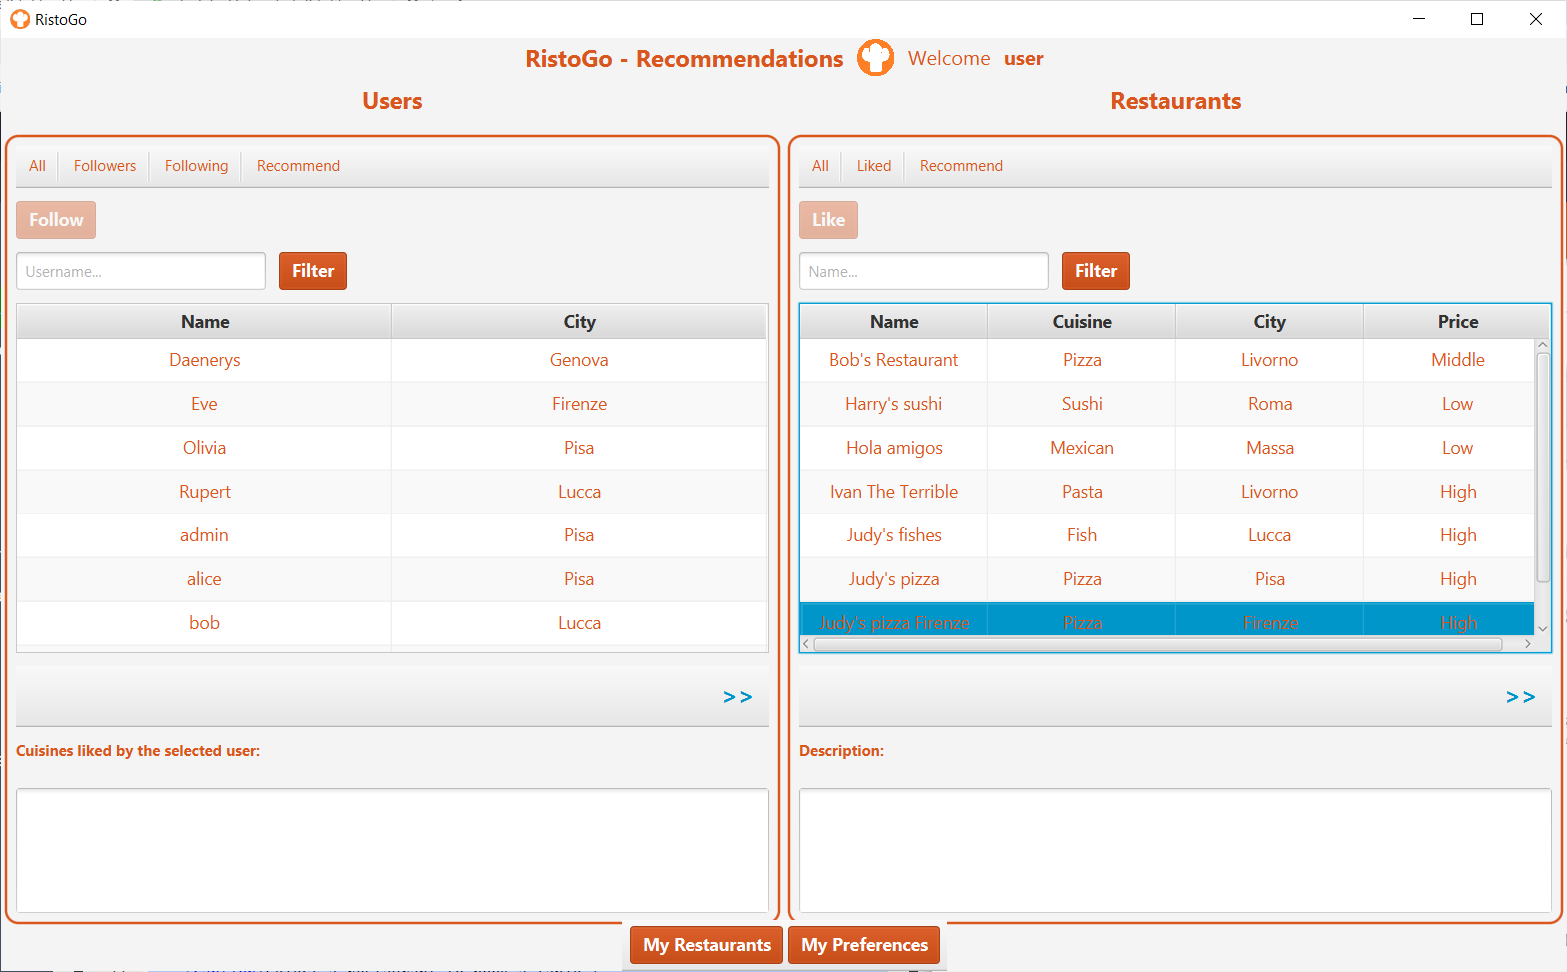
\includegraphics[width=\textwidth]{customer_interface}
	\caption{Customer interface.}\label{fig:customer_interface}
\end{figure}

\subsection{Follow users or put like to restaurants}

If you want to search particular users or restaurants, insert the name (or part
of the name) in the text field near the corresponding button ``Find'' and then
click it (\figref{fig:search}). Otherwise, don't do nothing and see the whole
list.

You can follow a user by selecting him (you can see also his/her favourite
cuisines) and clicking the button ``Follow''. If there are no errors you can see
the user in your following list.

You can put like to a restaurant by selecting it (you can see its description)
and clicking on the button ``Like''. If there are no errors you can see the user
in your like list.

\begin{figure}[H]
	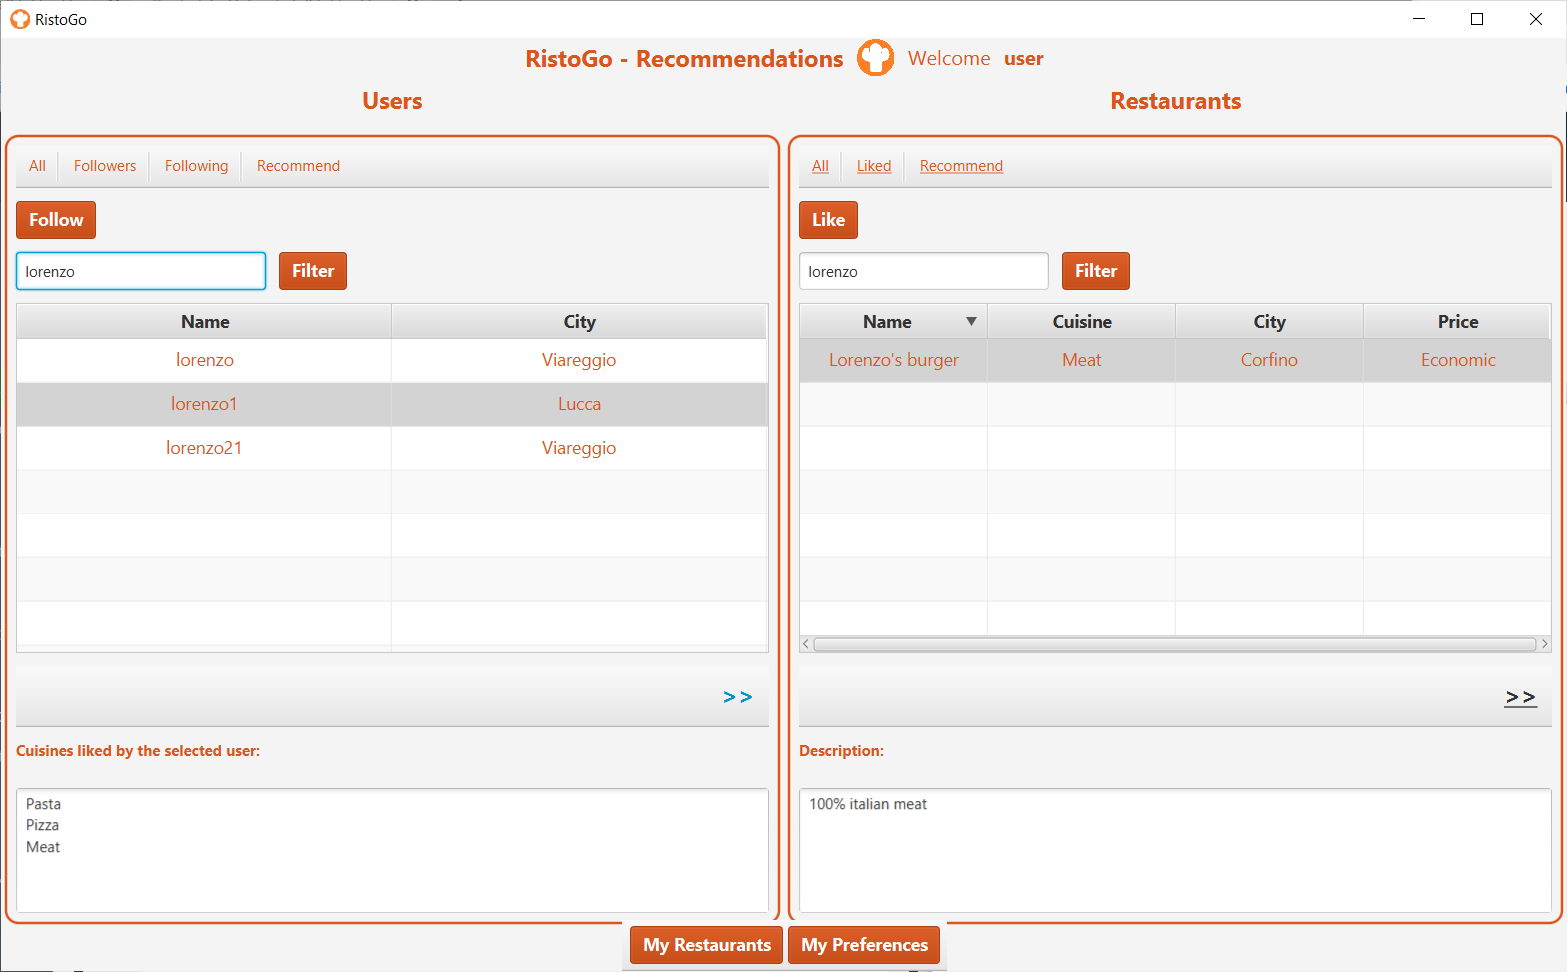
\includegraphics[width=\textwidth]{search}
	\caption{Search users or restaurants.}\label{fig:search}
\end{figure}

\subsection{Unfollow users}

In the user section, open the following list by clicking on ``following''. Here
you can find all the people that you follow. If you want, you can also see the
list of your followers clicking on ``followers'' (\figref{fig:following}).

Then, you can select one of your friends and click ``unfollow'' to stop
following him/her. If there are no errors, now you can't see the user in your
following list (\figref{fig:unfollow}).

\begin{figure}[H]
	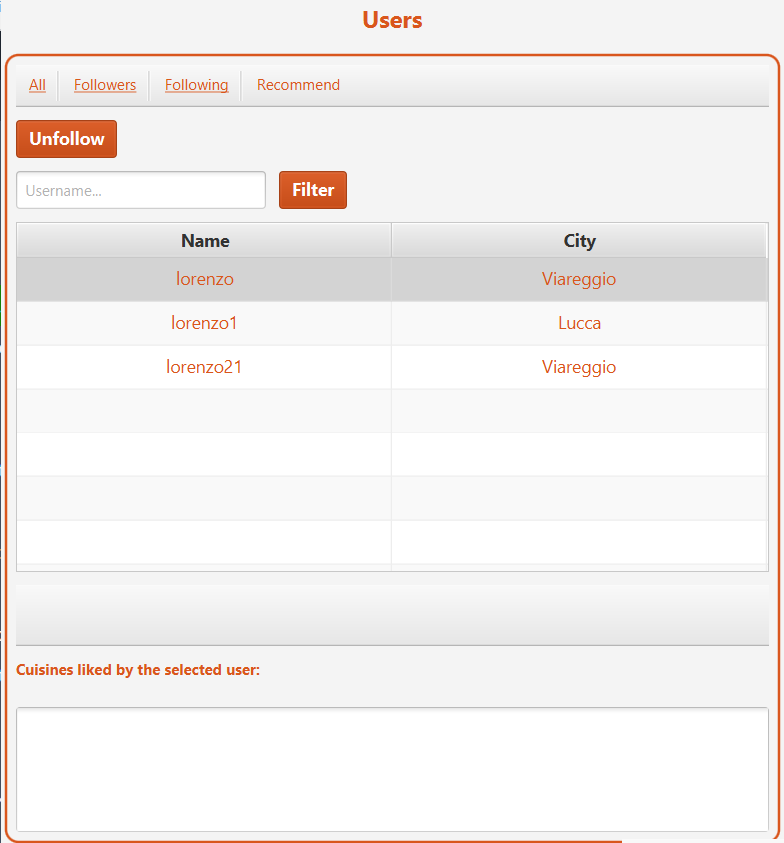
\includegraphics[width=\textwidth]{following}
	\caption{List of users followed.}\label{fig:following}
\end{figure}

\begin{figure}[H]
	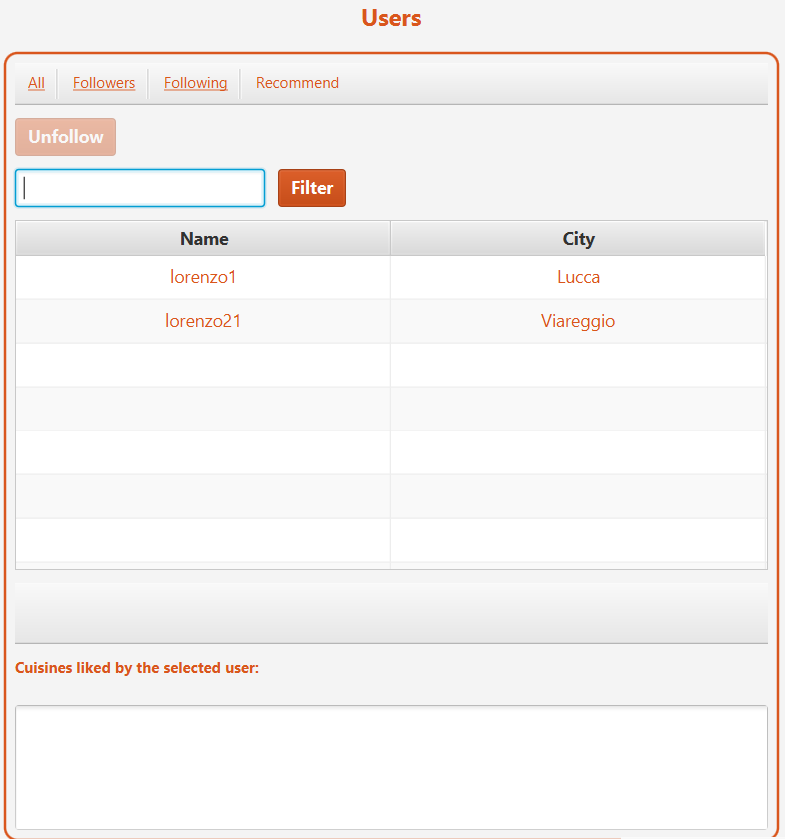
\includegraphics[width=\textwidth]{unfollow}
	\caption{List of users followed after an unfollow operation.}\label{fig:unfollow}
\end{figure}

\subsection{Unlike restaurants}

In the restaurant section, open the like list by clicking on ``liked''. Here you
can find all the restaurants that you like. (\figref{fig:like}).

Then, you can select one of your favourite restaurants and click ``unlike'' to
stop like it. If there are no errors, now you can't see the restaurant in your
like list (\figref{fig:unlike}).

\begin{figure}[H]
	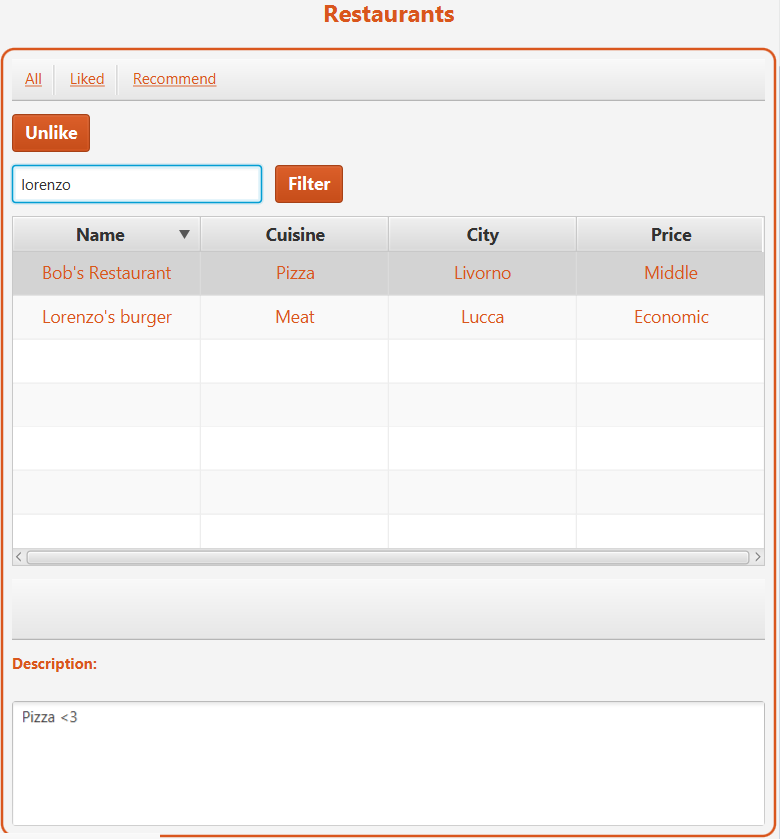
\includegraphics[width=\textwidth]{like}
	\caption{List of liked restaurants.}\label{fig:like}
\end{figure}

\begin{figure}[H]
	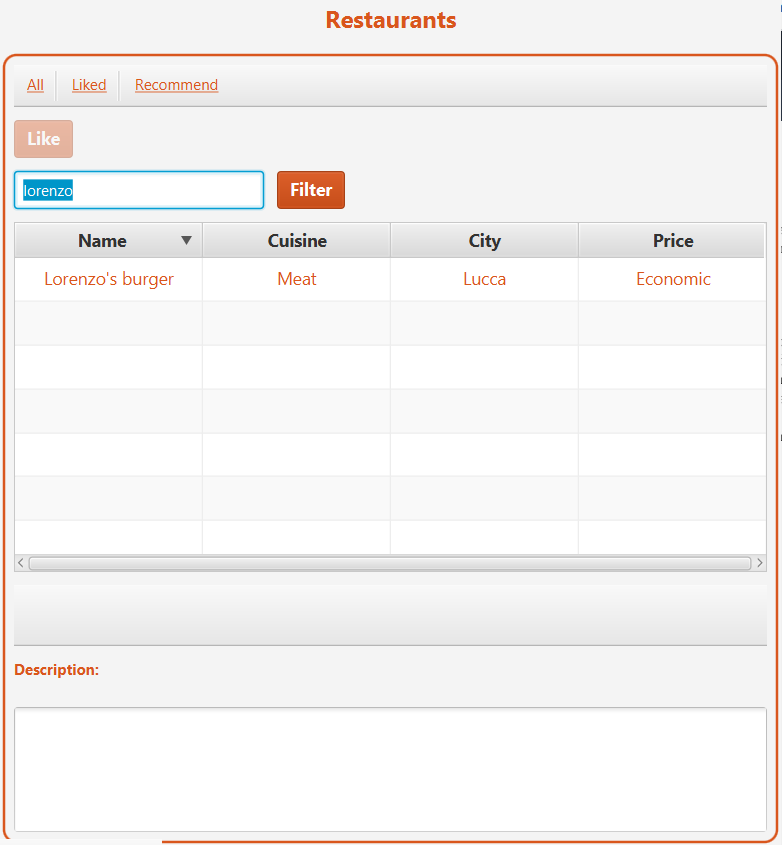
\includegraphics[width=\textwidth]{unlike}
	\caption{List of liked restaurants after an unlike operation.}\label{fig:unlike}
\end{figure}

\subsection{Friends recommendations}

In the user section, click on ``recommend'' to open the recommendation page
(\figref{fig:recommended_users}).

Then, select a city (by default it is the user city) and the maximum distance
from that city (if you want to search into all the cities, write a big value
such as \(10000\)). You can optionally select a type of cuisine. So you can
filter all the users that you are not already following, which are located into
a circle with center city and radius maximum distance, that likes the selected
cuisine, if specified (Figure~\ref{fig:filtered_users}).

\begin{figure}[H]
	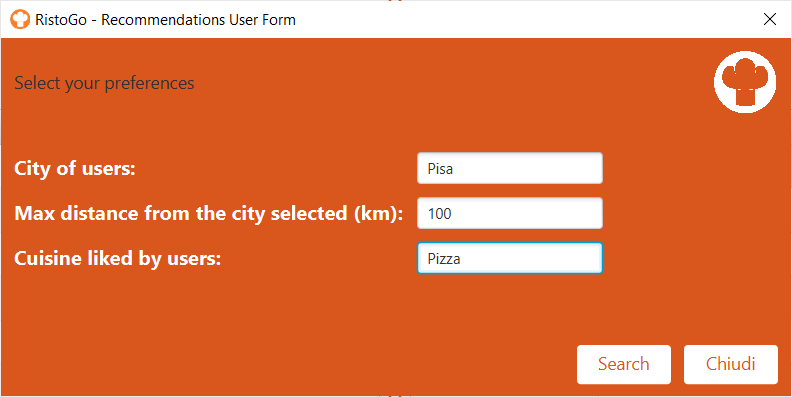
\includegraphics[width=\textwidth]{recommended_users}
	\caption{Form for users recommendations.}\label{fig:recommended_users}
\end{figure}

\begin{figure}[H]
	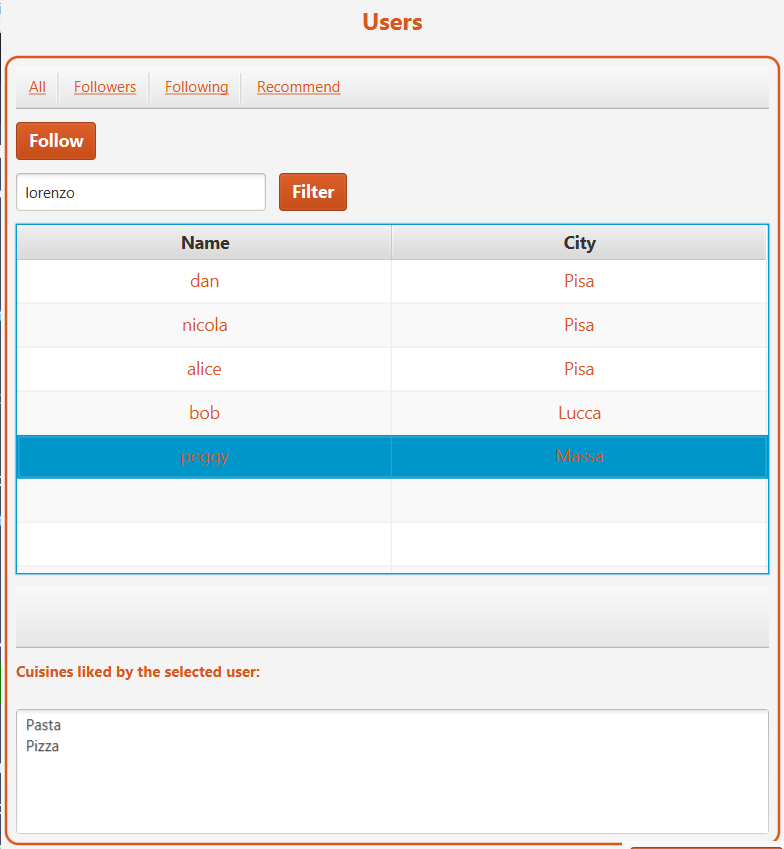
\includegraphics[width=\textwidth]{filtered_users}
	\caption{List of users after a recommendation operation.}\label{fig:filtered_users}
\end{figure}

\subsection{Restaurants recommendations}

In the restaurant section, click on ``recommend'' to open the recommendation
page (\figref{fig:recommended_restaurants}).

Then, select the order of likes (only friends or also friends of friends), a
city (by default it is the user city) and the maximum distance from that city
(if you want to search into all the cities, write a big value such as
\(10000\)). You can optionally select a type of cuisine. So you can filter all
the restaurants liked by the people you selected, that you are not already like,
which are located into a circle with center city and radius maximum distance,
that present the selected cuisine, if specified
(\figref{fig:filtered_restaurants}).

\begin{figure}[H]
	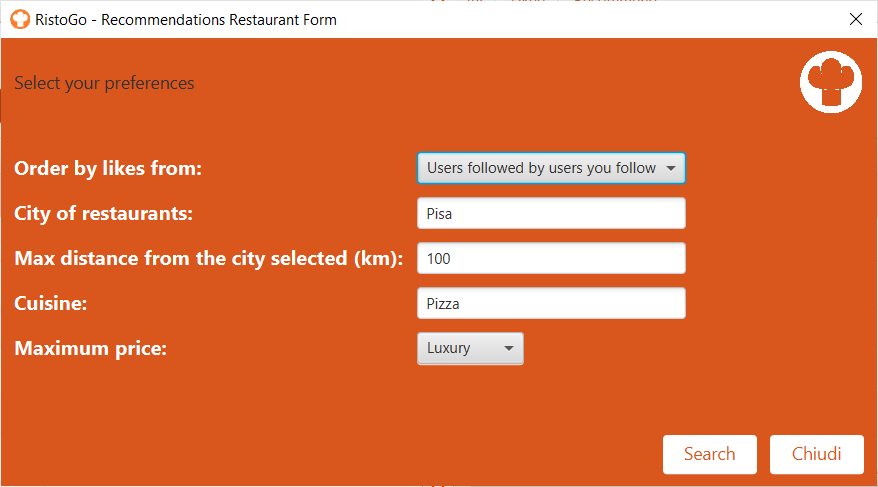
\includegraphics[width=\textwidth]{recommended_restaurants}
	\caption{Form for restaurants recommendations.}\label{fig:recommended_restaurants}
\end{figure}

\begin{figure}[H]
	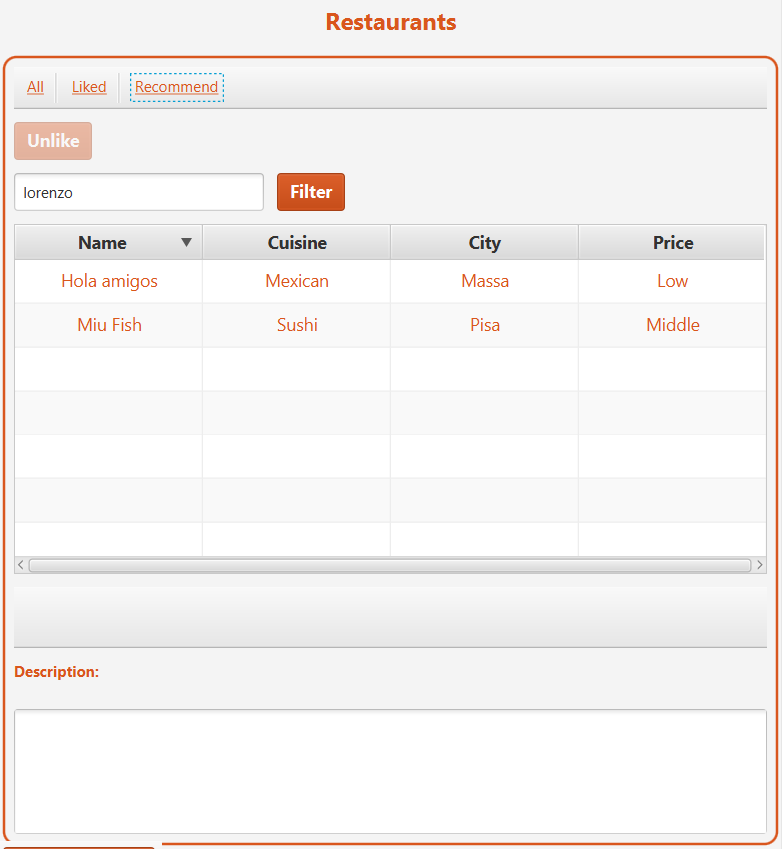
\includegraphics[width=\textwidth]{filtered_restaurants}
	\caption{List of restaurants after a recommendation operation.}\label{fig:filtered_restaurants}
\end{figure}

\subsection{Preferences}

In the main page, click on ``my preferences'' to see your residence city and
your favourite cuisines (\figref{fig:preferences}).

You can change your residence city typing the new one and clicking ``save''.

You can also add a new favourite cuisine writing it in the text field and
clicking ``add''. If there are no errors, you can see the new cuisine into the
preference list (\figref{fig:add_preferences}).

If you don't like anymore a cuisine you can delete it from your list selecting
it and clicking on ``remove''. If there are no errors, the city now isn't in
your preference list (\figref{fig:remove_preferences}).

\begin{figure}[H]
	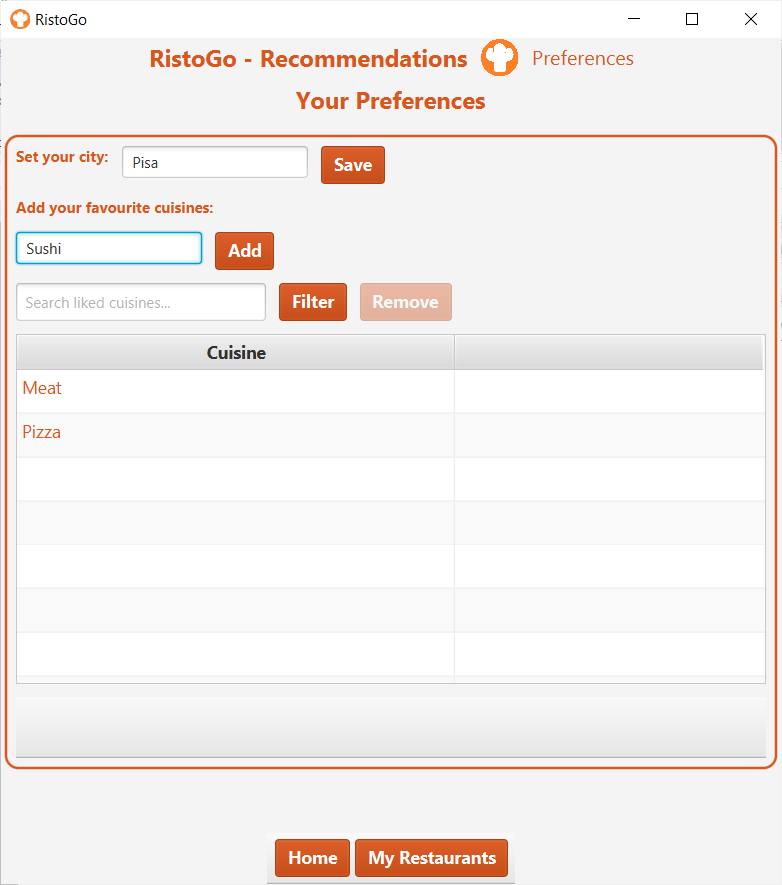
\includegraphics[width=\textwidth]{preferences}
	\caption{Preferences page.}\label{fig:preferences}
\end{figure}

\begin{figure}[H]
	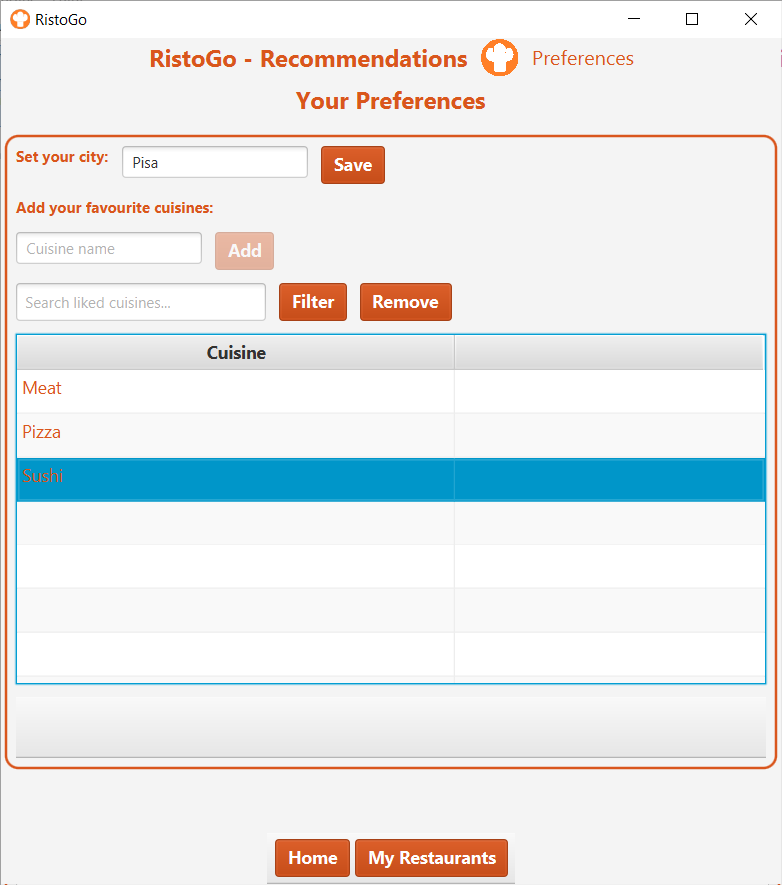
\includegraphics[width=\textwidth]{add_preferences}
	\caption{Preferences page after an add operation.}\label{fig:filtered_restaurants}
\end{figure}

\begin{figure}[H]
	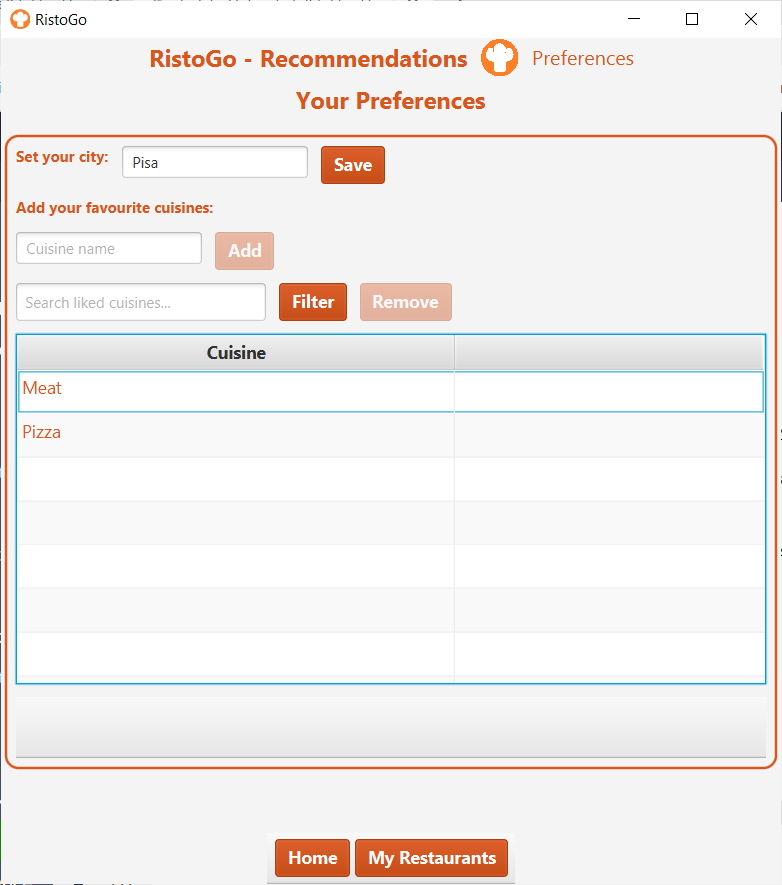
\includegraphics[width=\textwidth]{remove_preferences}
	\caption{Preferences page after a remove operation.}\label{fig:filtered_restaurants}
\end{figure}

\pagebreak
